\section{O Processo de Tomada de Decisão nas Organizações}

\begin{figure}[H]  % Use H para fixar a posição
    \centering
    \begin{minipage}{0.6\textwidth}
        \centering
        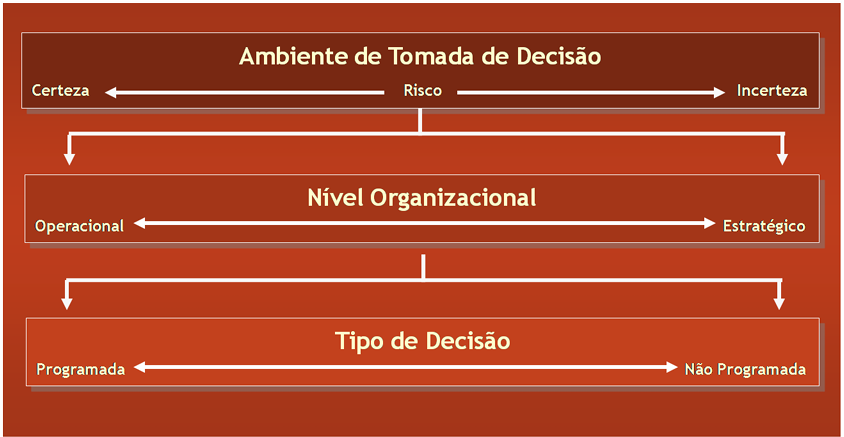
\includegraphics[width=\textwidth]{img/imagem5.png}
        \label{fig:exemplo}
    \end{minipage}
\end{figure}

O processo de tomada de decisão é uma parte fundamental da administração e impacta diretamente o desempenho das organizações. Diariamente, os administradores se deparam com inúmeras decisões, e a qualidade dessas escolhas influencia significativamente o sucesso da empresa. 

\textbf{O processo de tomada de decisão, geralmente aplicado a decisões não programadas, é composto por seis etapas:}

\begin{itemize}
    \item \textbf{Identificação da situação:} Reconhecimento de uma oportunidade, que permite à organização superar suas metas, ou de um problema, que surge quando o desempenho não é satisfatório e ameaça os objetivos da empresa.
    \item \textbf{Análise e diagnóstico da situação:} Definição dos objetivos a serem alcançados com a decisão e análise das causas que originaram a situação.
    \item \textbf{Desenvolvimento de alternativas:} Geração de diferentes cursos de ação que atendam às necessidades da situação e solucionem as causas subjacentes. É crucial \textbf{resistir à tentação de escolher a primeira opção viável} e \textbf{evitar analisar a viabilidade de cada alternativa à medida que surgem}, para garantir a exploração de todas as possibilidades.
    \item \textbf{Avaliação das alternativas:} Análise criteriosa das alternativas geradas, considerando fatores como custo, tempo, risco e impacto na organização. Diversas técnicas podem ser utilizadas nessa etapa, como a análise de prós e contras, a matriz de prioridades e as árvores de decisão.
    \item \textbf{Seleção e implementação:} Escolha da melhor alternativa, considerando os objetivos, valores da organização e a capacidade de solucionar o problema ou aproveitar a oportunidade. A implementação envolve ações como alocação de recursos, definição de cronogramas e comunicação da decisão aos envolvidos.
    \item \textbf{Monitoramento e feedback:} Acompanhamento da implementação da decisão e avaliação de sua eficácia na obtenção das metas. Essa etapa permite coletar informações e feedback para determinar se ajustes ou novas decisões são necessários.
\end{itemize}

\begin{figure}[H]  % Use H para fixar a posição
    \centering
    \begin{minipage}{0.8\textwidth}
        \centering
        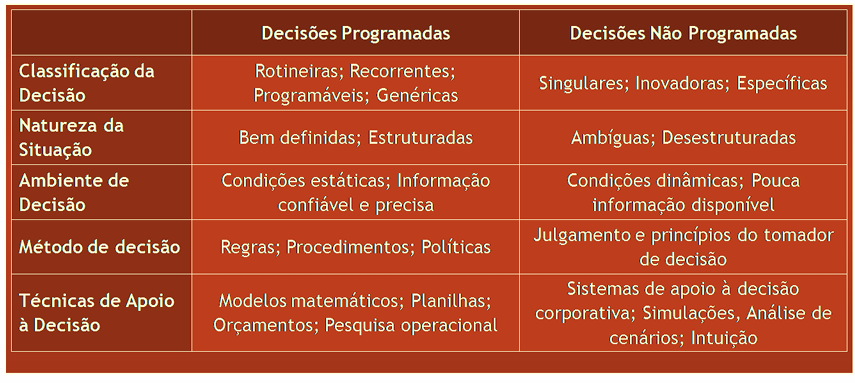
\includegraphics[width=\textwidth]{img/imagem6.png}
        \label{fig:exemplo}
    \end{minipage}
\end{figure}


\textbf{É importante observar que a tomada de decisão é um processo contínuo, que gera novos problemas e oportunidades, demandando novas decisões.}

\section{Racionalidade e Intuição na Tomada de Decisão}

O modelo racional de tomada de decisão descreve um processo ideal, no qual os administradores tomam decisões ótimas que maximizam os resultados da organização. No entanto, \textbf{na prática, a racionalidade total é raramente alcançada}.

\textbf{A teoria da racionalidade limitada de Herbert Simon reconhece que os administradores, na realidade, simplificam o processo decisório, considerando apenas os aspectos essenciais do problema, devido a restrições de tempo, recursos e capacidade cognitiva.} Em vez de buscar a solução ideal, os gestores buscam soluções satisfatórias que atendam a um nível aceitável de desempenho.

\textbf{Além das limitações contextuais, existem também armadilhas psicológicas que podem influenciar o julgamento dos administradores e levá-los a tomar decisões erradas.} Algumas dessas armadilhas são:
\begin{itemize}
    \item \textbf{Ancoragem:} Tendência a se apegar à primeira informação recebida, mesmo que irrelevante.
    \item \textbf{Perpetuação do status quo:} Favorecimento de alternativas que mantenham a situação atual.
    \item \textbf{Custo irrecuperável:} Persistência em decisões passadas, mesmo que equivocadas.
    \item \textbf{Evidência confirmadora:} Busca por informações que confirmem a própria opinião.
    \item \textbf{Formulação do problema:} A forma como o problema é apresentado pode influenciar a decisão.
    \item \textbf{Lembrança:} Tendência a supervalorizar eventos recentes ou marcantes.
    \item \textbf{Excesso de confiança:} Superestimação da própria capacidade de prever o futuro.
    \item \textbf{Prudência:} Estimativas e projeções excessivamente conservadoras.
\end{itemize}

\begin{figure}[H]  % Use H para fixar a posição
    \centering
    \begin{minipage}{0.6\textwidth}
        \centering
        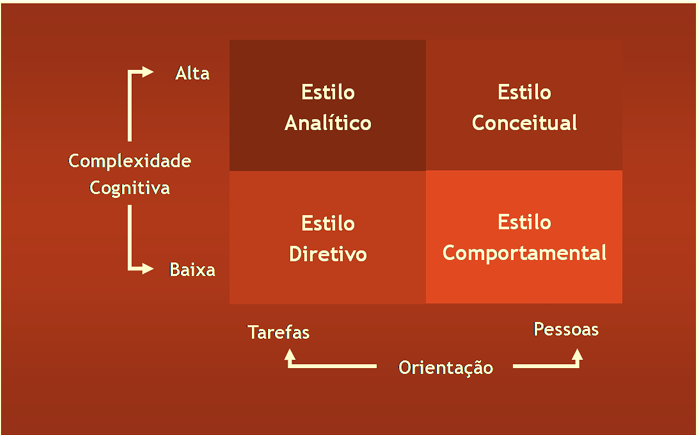
\includegraphics[width=\textwidth]{img/imagem7.png}
        \label{fig:exemplo}
    \end{minipage}
\end{figure}


\textbf{Apesar das limitações da racionalidade, a intuição também desempenha um papel importante na tomada de decisão.} A intuição pode ser definida como um processo de interpretação e conclusão sobre uma situação sem recorrer ao pensamento consciente, baseado em experiências e padrões mentais.

\textbf{A intuição pode ser útil em situações complexas ou com informações limitadas, mas é fundamental combiná-la com a análise racional para evitar decisões impulsivas.}

\textbf{Em resumo, o processo de tomada de decisão nas organizações é complexo e multifacetado, envolvendo tanto a racionalidade quanto a intuição. É crucial que os administradores compreendam os diferentes elementos que influenciam suas decisões, as limitações do modelo racional e as armadilhas psicológicas, para que possam tomar decisões mais eficazes e alcançar os objetivos da organização.}